\documentclass[12pt]{article}
\usepackage{tikz}

\begin{document}

\section{Introduction}

Rod Bogart suggested the idea of measuring the convexity of a geometric figure by picking two points uniformly at random within the figure and then asking for the probability that the straight line joining these points remains completely within the figure.
Equivalently we're asking for the probability that one point will be visible from the other.
For convex figures we will get a probability of $1$.
For non-convex figures where the ``defect'' from convexity is large enough to contain an open set we expect a probability less than $1$.
(I mention the open set because a disjoint union of a square and an isolated point will have a probability $1$ that the two points can be joined despite this set being non-convex.)

Rod used a Monte Carlo approach to compute the convexity of polyominoes.
I want to compute an exact expression for just one example, this polyomino:

\begin{center}
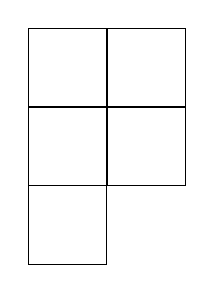
\begin{tikzpicture}
\draw[] (0,1) grid (2,3);
\draw[] (0,0) grid (1,1);
\end{tikzpicture}
\end{center}

\section{Basics}
Our problem is equivalent to this:
uniformly pick a pair of random squares in the polynomino and then pick a point uniformly in each polyomino.
What is the probability that one can see the other?
There are $5\times 5 = 25$ possible pairs.
Of these it should be clear that there are just 4 pairs of squares where there is any chance of visibility being blocked: $(A,B)$ and $(A, C)$ and their symmetric partners $(B,A)$ and $(C, A)$.

\begin{center}
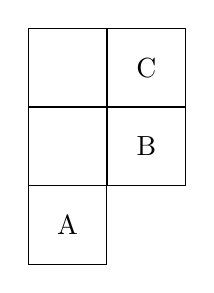
\begin{tikzpicture}
\draw[] (0,1) grid (2,3);
\draw[] (0,0) grid (1,1);
\draw (0.5, 0.5) node {A};
\draw (1.5, 1.5) node {B};
\draw (1.5, 2.5) node {C};
\end{tikzpicture}
\end{center}

\section{Can $A$ see $B$?}
Consider $(A,B)$ first.
The question we want to answer is this: if I pick a point uniformly in $A$ and another in $B$ will the second point be visible from the first?
Let's choose coordinates so the squares are all unit squares and the lower left corner is at $(0,0)$.
The issue is the corner at $(1,1)$.
If the line joining the two points falls below $(1,1)$ the view is blocked.
So one way of looking at the question is to ask this:
If the first point $p$ is picked uniformly in $A$, what fraction of $B$ falls under the line going through $p$ and $(1,1)$.

\begin{center}
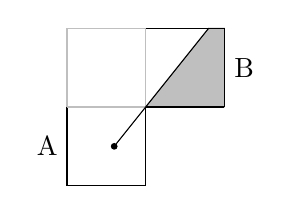
\begin{tikzpicture}
\filldraw [lightgray] (1,1)--(2,1)--(2,2)--(1.8,2.0)--(1,1);
\draw[] (1,1) grid (2,2);
\draw[] (0,0) grid (1,1);
\draw[lightgray] (0,1) grid (1,2);
\draw (-0.25, 0.5) node {A};
\draw (2.25, 1.5) node {B};
\filldraw (0.6, 0.5) circle (1pt);
\draw(0.6, 0.5) -- (1.8,2.0);
\end{tikzpicture}
\end{center}

The $(A,B)$ case is much easier than the $(A,C)$ case.
Pick $p$ in $A$ and $q$ in $B$ and note that if we reflect $p$ in the point $(1,1)$ to get $p'$, then $p'$ also falls on the line through $p$ and $(1,1)$.
So the question becomes, which line lies higher in square $B$, $(1,1)-p'$ or $(1,1)-q$.
By symmetry there is a $\frac{1}{2}$ chance of it being one or the other.
So a random point in $A$ has a $\frac{1}{2}$ of seeing a random point in $B$.

\section{Can $A$ see $C$?}

We now have to compute the area of the part of $C$ that is visible from points in $A$.
We can't use a simple symmetry argument here.
Let $p=(x',y')$ be the point in $A$.
Let's use coordinates $x, y$ such that $x=1-x'$ and $y=1-y'$.
There are three cases to consider
\begin{enumerate}
\item If $x>y$ then all of $C$ is visible.
\item if $\frac{1}{2}y<x<y$ then there is a triangle in $C$ that is occluded.
\item if $x<\frac{1}{2}y$ then a trapezium in $C$ is occluded.
\end{enumerate}
To compute the overall probability that there is occlusion between a point in $A$ and a point in $C$ we need to integrate the area of the occluded region for all $(x',y')$ in the unit square, or equivalently, for all $(x,y)$ in the unit square.
We break this up into three pieces according to the three cases.

\subsection{Case 1}
For $x>y$ the occluded region in $C$ has zero area.

\subsection{Case 2}
\begin{center}
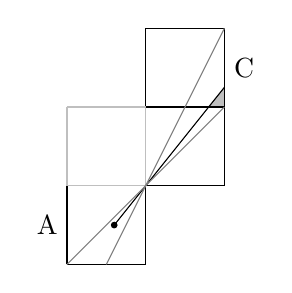
\begin{tikzpicture}
\filldraw [lightgray] (1.8,2.0)--(2,2)--(2,2.25)--(1.8,2.0);
\draw[] (1,1) grid (2,3);
\draw[] (0,0) grid (1,1);
\draw[lightgray] (0,1) grid (1,2);
\draw (-0.25, 0.5) node {A};
\draw (2.25, 2.5) node {C};
\filldraw (0.6, 0.5) circle (1pt);
\draw(0.6, 0.5) -- (2.0,2.25);
\draw [gray] (0.5,0)--(2,3);
\draw [gray] (0.0,0)--(2,2);
\end{tikzpicture}
\end{center}

The occluded triangle has corners: $(1+x/y,2), (2,1+y/x), (2,2)$.
This has area $\frac{1}{2}\left(1-\frac{x}{y}\right)\left(\frac{y}{x}-1\right)$.

We need to integrate this over the subregion $y/2<x<y$ in the unit square.

\[
I =
\int_0^1 \int_{y/2}^y \frac{1}{2}\left(1-\frac{x}{y}\right)\left(\frac{y}{x}-1\right)  dxdy
= \int_0^1 \left(-\frac{5}{16}+\frac{1}{2}\log 2\right)y  dy
= -\frac{5}{32}+\frac{\log 2}{4}
\]

\subsection{Case 3}
\begin{center}
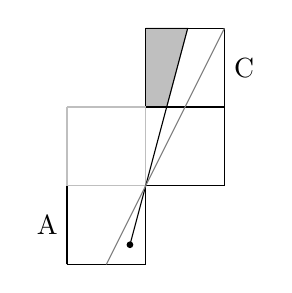
\begin{tikzpicture}
\filldraw [lightgray] (1,3)--(1,2)--(1.26667,2)--(1.53333,3)--(1,3);
\draw[] (1,1) grid (2,3);
\draw[] (0,0) grid (1,1);
\draw[lightgray] (0,1) grid (1,2);
\draw (-0.25, 0.5) node {A};
\draw (2.25, 2.5) node {C};
\filldraw (0.8, 0.25) circle (1pt);
\draw(0.8, 0.25) -- (1.5333,3);
\draw [gray] (0.5,0)--(2,3);
\end{tikzpicture}
\end{center}

We have a trapezium with corners: $(1,2), (1+x/y,2), (1+2x/y,3), (1,3)$.
Its area is $1-3x/2y$.

We need to integrate this over the subregion of the unit square where $x < y/2$.

\[
J =
\int_0^1 \int_0^{y/2} \left(1-\frac{3x}{2y}\right) dxdy
= \int_0^1 \frac{5ydy}{16}
= \frac{5}{32}
\]

\section{The grand total}
Out of 25 pairs of squares, only 4 have any kind of occlusion.
In the case of $(A,B)$ and $(B,A)$ we have a $\frac{1}{2}$ chance of occlusion.
In the case of $(A,C)$ and $(C,A)$ we have a probability $I+J$ of occlusion.
Putting it all together we have a probability that the first point can view the second point given by
\[
1-\frac{1}{25}(2\frac{1}{2}+2(I+J)) = \frac{1}{50}(48-\log 2) = 0.946137
\]

\end{document}
